% Copyright (C) 2018 by latexstudio <http://www.latexstudio.net>
%
% This program is free software: you can redistribute it and/or modify
% it under the terms of the GNU General Public License as published by
% the Free Software Foundation, either version 3 of the License, or
% (at your option) any later version.
%
% This program is distributed in the hope that it will be useful,
% but WITHOUT ANY WARRANTY; without even the implied warranty of
% MERCHANTABILITY or FITNESS FOR A PARTICULAR PURPOSE.  See the
% GNU General Public License for more details.
%
% You should have received a copy of the GNU General Public License
% along with this program.  If not, see <http://www.gnu.org/licenses/>.
%

\section{字体篇}


\faq{LaTeX字体是如何处理的}{}

LaTeX 2ε目前的字体机制称为``新字体选择机制''(New Font Selection
Scheme,NFSS)。它将文本字体分为五个互不干扰的属性(数学字体初学者不必过早了解):
\begin{enumerate}
  \item
    编码(encoding)。这个属性初学者暂时不必了解。在(pdf)latex和uplatex中,默认的西文编码称为OT1;在xelatex中,默认的编码称为EU2,就是Unicode。
  \item
    字族(family)。一套成风格的字型的统称,如cmr、ptm(times)等。\LaTeXe{}
    预先定义了三个切换字族的命令:\cs{rmfamily}(衬线体)、\cs{sffamily}(无衬线体)、\cs{ttfamily}(等宽体)。
  \item
    系列(series)。在一般的字体中一般表示字重(weight)。如粗体命令为\cs{bfseries},正常粗细为\cs{mdseries}。
  \item
    字形(shape)。在同一字族、同一系列下的风格差异,如斜体\cs{slshape}、意大利斜体\cs{itshape}、正体\cs{upshape}、小型大写\cs{scshape}。
  \item
    字号(size)。以上四种变化是字型(typeface)的变化,而这是同一字型下不同大小的变化。LaTeX
    2ε提供了成套的字号命令,如\cs{normalsize}、\cs{small}、\cs{scriptsize} 等。
\end{enumerate}

中文字体的方面,不同的中文解决方案的处理也有不同,这里就不介绍了。


\faq{获取位图字体}{}


\faq{PDF格式图片插入过程中的字形缺失}{}


\faq{为数学排版选择Type 1字体}{}


\faq{Type 1字体配置}{}


\faq{切换到T1时字体变得模糊}{}


\faq{由于Ghostscript太旧造成字体模糊}{}


\faq{如何使用斜体}{}

斜体一般是西文字体用的,在中文中不用斜体。

斜体这个名字比较误导,因为它对应英文的两个名字:倾斜体(slanted,指字形风格大致相同但是倾斜)和意大利体(italic,指字形设计为接近手写的形态,同时也就出现了倾斜)。

两种情况下分别有 \cs{slshape} 和 \cs{itshape} 两个命令,使用例如
|{\slshape slanted}| 及|{\itshape italic}|;也有把斜体内容作为参数的命令(推荐使用这种),如\textsl{slanted}及\textit{italic}。


\faq{如何使用粗体}{}

\begin{enumerate}
\def\labelenumi{\arabic{enumi}.}
\item
  \cs{mathbf}

  \cs{mathbf}
  会将数学模式取消再来取用字型,因此它加粗的不是数学符号,而是公式里的一般文字。\cs{mathbf} 只能在公式内部使用:
\end{enumerate}

\begin{verbatim}
\documentclass{article}
\begin{document}
$\mathbf{equation: f(x,y) = \alpha x^2 + \beta y^2}$
\end{document}
\end{verbatim}

效果如下:
% \includegraphics{https://images-cdn.shimo.im/tmTzWYcpaSUPPQCQ/image.png!thumbnail}

\begin{enumerate}
\def\labelenumi{\arabic{enumi}.}
\setcounter{enumi}{1}
\item
  \cs{boldmath}

  \cs{boldmath} 可以将整套数学字体切换为粗体版本,这个命令只能在公式外使用:
\end{enumerate}

\begin{verbatim}
\documentclass{article}
\begin{document}
\boldmath{$f(x,y) = \alpha x^2 + \beta y^2$}
\end{document}
\end{verbatim}

效果如下:
% \includegraphics{https://images-cdn.shimo.im/FT1utRInpn8FWCZX/image.png!thumbnail}

\begin{enumerate}
\def\labelenumi{\arabic{enumi}.}
\setcounter{enumi}{2}
\item
  \cs{boldsymbol}

  amsmath 提供了一个 \cs{boldsymbol} 命令(由调用的 amsbsy
  宏包提供),用于打破 \cs{boldmath}
  的限制,在公式内部将一部分符号切换为粗体:
\end{enumerate}

\begin{verbatim}
\documentclass{article}
\usepackage{amsbsy}%或者直接调用常用宏包amsmath
\begin{document}
$f(x,y) = \boldsymbol{\alpha x^2 + \beta y^2}$
\end{document}
\end{verbatim}

效果如下:
% \includegraphics{https://images-cdn.shimo.im/FiwJiO2EZeYTf4j7/image.png!thumbnail}

\begin{enumerate}
\def\labelenumi{\arabic{enumi}.}
\setcounter{enumi}{3}
\item
  \cs{bm}
\end{enumerate}

\begin{verbatim}
\documentclass{article}
\usepackage{bm}
\begin{document}
$\sum x_i y_i$,
$\bm{\sum x_i y_i}$,
${\bm \sum}{\bm x_i}{\bm y_i}$.
\end{document}
\end{verbatim}

效果如下:
% \includegraphics{https://images-cdn.shimo.im/yKpDot5b9oUc6ww3/image.png!thumbnail}

\begin{enumerate}
\def\labelenumi{\arabic{enumi}.}
\setcounter{enumi}{4}
\item
  \cs{pmb}

  需使用 amamath 宏包。
\item
  \textbf
  文本加粗
\end{enumerate}

\begin{verbatim}
\documentclass{article}
\begin{document}
\textbf{equation: $f(x,y)=\alpha x^2+\beta y^2$}
\end{document}
\end{verbatim}

效果如下:
% \includegraphics{https://images-cdn.shimo.im/ZFmJXLZAIGQKq0VQ/image.png!thumbnail}

\begin{enumerate}
\def\labelenumi{\arabic{enumi}.}
\setcounter{enumi}{6}

\item
  \cs{bfseries}
  \cs{bfseries} 影响之后所有的字符,如果想让它在局部生效,需使用花括号分组:
\end{enumerate}

\begin{verbatim}
\documentclass{article}
\begin{document}
{\bfseries equation: $f(x,y) = \alpha x^2 + \beta y^2$}\\
equation: $f(x,y) = \alpha x^2 + \beta y^2$.\\
\bfseries equation: $f(x,y) = \alpha x^2 + \beta y^2$\\
equation: $f(x,y) = \alpha x^2 + \beta y^2$.\\
\end{document}
\end{verbatim}

效果如下:
% \includegraphics{https://images-cdn.shimo.im/rafHmr9a7JYYebWs/image.png!thumbnail}
参考: Ishort-zh-cn LaTeX入门,刘海洋。
\url{http://blog.sina.com.cn/s/blog_5e16f1770100nqwx.html}


\faq{如何设置文档字体为本机已安装字体?}{}


\faq{如何通过字体文件名来调用未安装本机字体?}{}


\faq{字体大小经常出现警告,该引用什么宏包解决?}{}


\faq{有些特殊文字怎么加入Latex文档,例如symbol\{"ff0e\}编译后为空白}{}


\faq{如何查看字体和行间距,然后怎样修改}{}


\faq{字体相对大小指令}{}

\cs{small} 等命令对应的字体大小与文章 \cs{documentlcass} 中指定的字体有关,对应
10, 11, 12pt 三种全局字体大小的情况如下表所示, 指令 10pt 11pt 12pt
% \tiny                           5 6 6
% \scriptsize                 7 8 8
% \footnotesize            8 9 10
% \small                        9 10 10.95
% \normalsize              10 10.95 12
% \large                       12 12 14.4
% \Large                      14.4 14.4 17.28
% \LARGE                    17.28 17.28 20.74
% \huge                       20.74 20.74 24.88
% \Huge                      24.88 24.88 24.88


\faq{在latex公式中如何将某一个字母或者希腊符号设置成某一个字体?}{}
